% \documentclass{article}
% \usepackage[margin=1cm]{graphicx} % Required for inserting images
% \usepackage[russian]{babel}
% \usepackage{caption}
% \usepackage{geometry}
% \usepackage{url}
% \usepackage{amsfonts}
% \usepackage{amsmath}
% \usepackage{float}
% \usepackage[a4paper, top=2cm, bottom=3cm, left=3cm, right=1cm]{geometry}
\documentclass[a4paper,12pt]{article}
\usepackage[utf8]{inputenc}
\usepackage[russian]{babel}
\usepackage{amsmath}
\usepackage{multicol}
\usepackage{url}
\usepackage[margin=1cm]{graphicx} % Required for inserting images
\usepackage[a4paper, top=2cm, bottom=3cm, left=1cm, right=2cm]{geometry}

\title{Санкт-Петербургский политехнический университет
Петра Великого
Физико-механический институт
Высшая школа прикладной математики и вычислительной
физики}
\date{}
\begin{document}

\maketitle
\begin{center}
{\fontsize{25}{}\selectfont Отчёт \\
по лабораторной работе №2 \\
по дисциплине \\
«Интервальный анализ»}

\end{center}
\begin{flushright}
Выполнил студент:\\
Басалаев Даниил
группа:\\
5030102/10201\\

\end{flushright}

\vspace*{\fill} \begin{center}Санкт-Петербург\end{center}

\newpage % Начать новую страницу для содержания
\tableofcontents

\newpage
\section{Постановка задачи}
Решение линейной задачи о допусках\\
Дан набор ИСЛАУ (1)
$$\boldsymbol{A_i}\cdot x=\boldsymbol{b_i}, \;\;\; x = (x_1, x_2)\eqno(1)$$
c матрицей (2) и вектором правой части (3)
\[ A_1 =
 \begin{pmatrix}
    [0.65, 1.25] & [0.70, 1.3] \\
    [0.75, 1.35] & [0.70, 1.3] 
 \end{pmatrix} \:\:
 A_2 =
 \begin{pmatrix}
    [0.65, 1.25] & [0.70, 1.3] \\
    [0.75, 1.35] & [0.70, 1.3] \\
    [0.8, 1.4] & [0.70, 1.3]
 \end{pmatrix} \;\;
 A_3 =
 \begin{pmatrix}
    [0.65, 1.25] & [0.70, 1.3] \\
    [0.75, 1.35] & [0.70, 1.3] \\
    [0.8, 1.4] & [0.70, 1.3] \\
    [−0.3, 0.3] & [0.70, 1.3]
 \end{pmatrix}
  \eqno(2)
\]

\[
b_1 = 
\begin{pmatrix}
    [2.75, 3.15]\\
    [2.85, 3.25]
\end{pmatrix} \;\;
b_2 = 
\begin{pmatrix}
    [2.75, 3.15] \\
    [2.85, 3.25] \\
    [2.90, 3.3] \\
\end{pmatrix}\;\;
b_3 = 
\begin{pmatrix}
    [2.75, 3.15] \\
    [2.85, 3.25]\\
    [2.90, 3.3]\\
    [1.8, 2.2]\\
\end{pmatrix}
  \eqno(3)
\]
\\\\
\textbf{Задание}
\begin{enumerate}
    \item Проверить непустоту допускового множества ИСЛАУ (1)
    \item Построить график функционала $Tol (x)$ для (1)
    \item Построить допусковое множество ИСЛАУ (1)
    \item Найти argmax Tol и образующие допускового функционала
\end{enumerate}\\\\
Для достижения непустого допускового множества провести коррекцию ИСЛАУ (1):
\begin{enumerate}
    \item правой части ИСЛАУ (3) — b-коррекция
    \item матрицы ИСЛАУ (2) — A-коррекция
    \item комбинацией предыдущих методов с одновременным изменением правой части и матрицы ИСЛАУ — Ab-коррекция
\end{enumerate}\\
\\Для всех видов коррекции построить график функционала $Tol (x)$, допускового множества, отобразить argmaxTol и найденные ранее частные решения набора СЛАУ


\newpage
\section{Теоретическое обоснование}
\textbf{Некоторые необходимые формулы:}
\begin{itemize}
    \item \textit{Середина интервала}
    \begin{equation*}
 mid \textbf{ a}=(\overline{\textbf{a}}+\textbf{\underline{a}})/2
 \end{equation*}
    \item \textit{Радиус интервала}
    \begin{equation*}
 rad \textbf{ a}=(\overline{\textbf{a}}-\textbf{\underline{a}})/2
 \end{equation*}
    \item \textit{Магнитудой (aбсолютной величиной, модулем) интервала} называется наибольшее из абсолютных значений точек интервала \textbf{a}:
    \begin{equation*}
 \textbf{ a}:=\max\{|a|\textbf{ | } a \in \textbf{a}\}=\max\{|\textbf{\underline{a}}|, |\overline{\textbf{a}}|\}
 \end{equation*}
\end{itemize}
\\
\textbf{def.} Допусковое множество решений:
\begin{equation}\tag{1.1}
 \Xi_{tol}(\textbf{A, b})=\{x \in \mathbb{R}^n|(\forall A \in \textbf{A})(\exists b \in \textbf{b})(Ax=b)\}
 \end{equation}
\\
\textbf{Теорема 1.} Пусть даны интервальная $m \times n$-матрица \textbf{A} и интервальный вектор правой части \textbf{b}, а выражением
\begin{equation}\tag{1.2}
 Tol(x, \textbf{A, b})=\min_{1\leq i\leq m}\lbrace rad \text{ }b_i - \lvert mid \text{ }b_i - \sum_{j=1}^{n}a_{ij}x_j \rvert \rbrace 
 \end{equation}
определяется функционал $Tol$ : $\mathbb{R}^n\times\mathbb{IR}^{m\times n}\times \mathbb{IR}^m\rightarrow \mathbb{R}$. Тогда принадлежность $x \in \Xi_{tol}(\textbf{A,b})$ равносильна $Tol(x,\textbf{A, b}) \geq 0$, допусковое
множество решений интервальной линейной системы $\textbf{A}x=\textbf{b}$ есть множество уровня
\begin{equation*}
 \{x \in \mathbb{R}^n \textbf{ }|\textbf{ } Tol(x,\textbf{A, b}) \geq 0\}
 \end{equation*}
функционала Tol.
\\
\\
\textbf{Решение ЛЗД(линейной задачи о допусках) можно разделить на следующие этапы:}
\begin{enumerate}
    \item исследование разрешимости ЛЗД, в результате проведения которого делается вывод о пустоте/непустоте допускового множества решений $\Xi_{tol}(\textbf{A, b})$ ИСЛАУ,
    \item  коррекция ЛЗД, выполняемая с целью достичь разрешимости поставленной интервальной задачи,
    \item построение бруса решения ЛЗД.
\end{enumerate}
\\
\textbf{def.} Процедура изменения входных данных ЛЗД(линейной задачи о допусках) для достижения ее совместности называется коррекцией.\\
\\
\\Дальше рассмотрим подробно каждый вид коррекции.
\subsection{b-коррекция: коррекция правой части}
Первый, технически более простой, подход к достижению разрешимости ЛЗД заключается в коррекции вектора \textbf{b} и направлен на ослабление ограничений в правой части ИСЛАУ, т. е. расширение допусков.\\
\\
\textbf{Равномерное уширение всех компонент вектора правой части
ИСЛАУ}\\
Пусть матрица \textbf{A} ИСЛАУ неизменна, и значения $mid$ $b_i$, $m=1,2,\dots,m$ зафиксированы. Тогда расширение вектора \textbf{b} путем его замены на вектор
\begin{equation*}
\textbf{b} + Ke, \textbf{ }K ≥ 0,\textbf{ }e =(︀[−1, 1], . . . , [−1, 1])︀^T
 \end{equation*}
приведет к тому, что значение абсолютного максимума $T$ распознающего функционала $Tol(x,\textbf{A, b})$ возрастет на постоянную $K$:
\begin{equation*}
\max_{x \in \mathbb{R}^n}Tol(x, \textbf{A, b}+Ke)=\max_{x \in \mathbb{R}^n}Tol(x, \textbf{A, b})+K=T+K
\end{equation*}
причем Arg max Tol — положение точки $T$ — не изменится.
\\

\subsection{A-коррекция}
Рассмотрим интервальную матрицу \textbf{A} ИСЛАУ, для которой имеет место
\begin{equation*}
    rad \text{ }\mathbf{b}_i>0 \text{ и } \sum_{j=1}^{n}rad\text{ }\mathbf{a}_{ij}>0,\text{ }i=1,2,\dots,m.
\end{equation*}
Идея коррекции матрицы \textbf{A} ИСЛАУ заключается в том, чтобы заменить ее интервальной матрицей
  \( \mathbf{A} \ominus \mathbf{E} \) такой, что
  \[
    \text{rad} (\mathbf{A} \ominus \mathbf{E}) < \text{rad} \mathbf{A}, \]
   \[\text{mid} (\mathbf{A} \ominus \mathbf{E}) = \text{mid} \mathbf{A} \]
и тем самым достичь разрешимости ЛЗД для ИСЛАУ с интервальными
матрицей \( \mathbf{A} \ominus \mathbf{E} \) и неизменным вектором правой части $\mathbf{b}$.\\
Операция, обозначаемая через «$\ominus$», называется внутренним вычитанием в полной интервальной арифметике Каухера $\mathbb{KR}$:
\begin{equation*}
    a \ominus b:=[\underline{\mathbf{a}}-\underline{\mathbf{b}},\overline{\mathbf{a}}-\overline{\mathbf{b}}]
\end{equation*}
Матрица $\mathbf{E}$, которая вычитается с помощью операции «$\ominus$» из матрицы $\mathbf{A}$ исходной ИСЛАУ, является матрицей размера $m \times n$ с уравновешенными интервальными элементами $\mathbf{e}_{ij} = [-e_{ij}, e_{ij}]$, причем значения точечных величин $e_{ij}$ удовлетворяют двум условиям:
  \[
    0 \leq e_{ij} \leq rad \text{ }\mathbf{a}_{ij} \text{ для всех i, j,} \]
   \[\sum_{j=1}^{n}e_{ij}|\tau_j|=K, \text{ }i=1,2,\dots,m \]
где $K$— положительная постоянная, $\tau_j$ ,$j=1,2,\dots,n$ — аргументы безусловного максимума распознающего функционала $Tol(x,\textbf{A, b})$.

\subsection{Ab-коррекция}
\( Ab \)-коррекцией ИСЛАУ \( \mathbf{A}x = \mathbf{b} \) заключается
  в комбинированном применении \( A \)-коррекци и \( b \)-коррекции.
  Этапы $Ab$-коррекции:
  \begin{enumerate}
      \item Сужение элементов матрицы \( \mathbf{A} \) с помощью $A$-коррекции
      \item Расширение вектора правой части \( \mathbf{b} \) с помощью $b$-коррекции
  \end{enumerate}


\section{Результат}
\subsection{Без коррекции}
Если не проводить коррекцию, то для каждого случае (1), (2) получаем, что максимальное значение функционала $Tol(x, \mathbf{A}, \mathbf{b})$ отрицательно и равно -0,7 и допусковое множество пусто.

\begin{center}
\begin{tabular}{|c|c|c|c|}
\hline
$\mathbf{A}$&$\mathbf{b}$&$max{Tol(x, \mathbf{A}, \mathbf{b})}$& $argmax{Tol(x, \mathbf{A}, \mathbf{b})}$\\
\hline
$\begin{pmatrix}
    [0.65, 1.25] & [0.70, 1.3] \\
    [0.75, 1.35] & [0.70, 1.3]
\end{pmatrix}$&\begin{pmatrix}
    [2.75, 3.15] \\
    [2.85, 3.25]
\end{pmatrix}&-0.7000000000000004&[1,2]\\
\hline
\begin{pmatrix}
    [0.65, 1.25] & [0.70, 1.3] \\
    [0.75, 1.35] & [0.70, 1.3] \\
    [0.8, 1.4] & [0.70, 1.3]
\end{pmatrix}
&\begin{pmatrix}
    [2.75, 3.15] \\
    [2.85, 3.25]\\
    [2.90, 3.3]
\end{pmatrix}&-0.7000000000000013&[1,2]\\
\hline
$\begin{pmatrix}
    [0.65, 1.25] & [0.70, 1.3] \\
    [0.75, 1.35] & [0.70, 1.3] \\
    [0.8, 1.4] & [0.70, 1.3] \\
    [-0.3, 0.3] & [0.70, 1.3]
\end{pmatrix}$&$\begin{pmatrix}
    [2.75, 3.15] \\
    [2.85, 3.25]\\
    [2.90, 3.3] \\
    [1.8,2.2]
\end{pmatrix}$&-0.7000000000000022&[1,2]\\
\hline
\end{tabular}
\end{center}

\begin{figure}[htp]
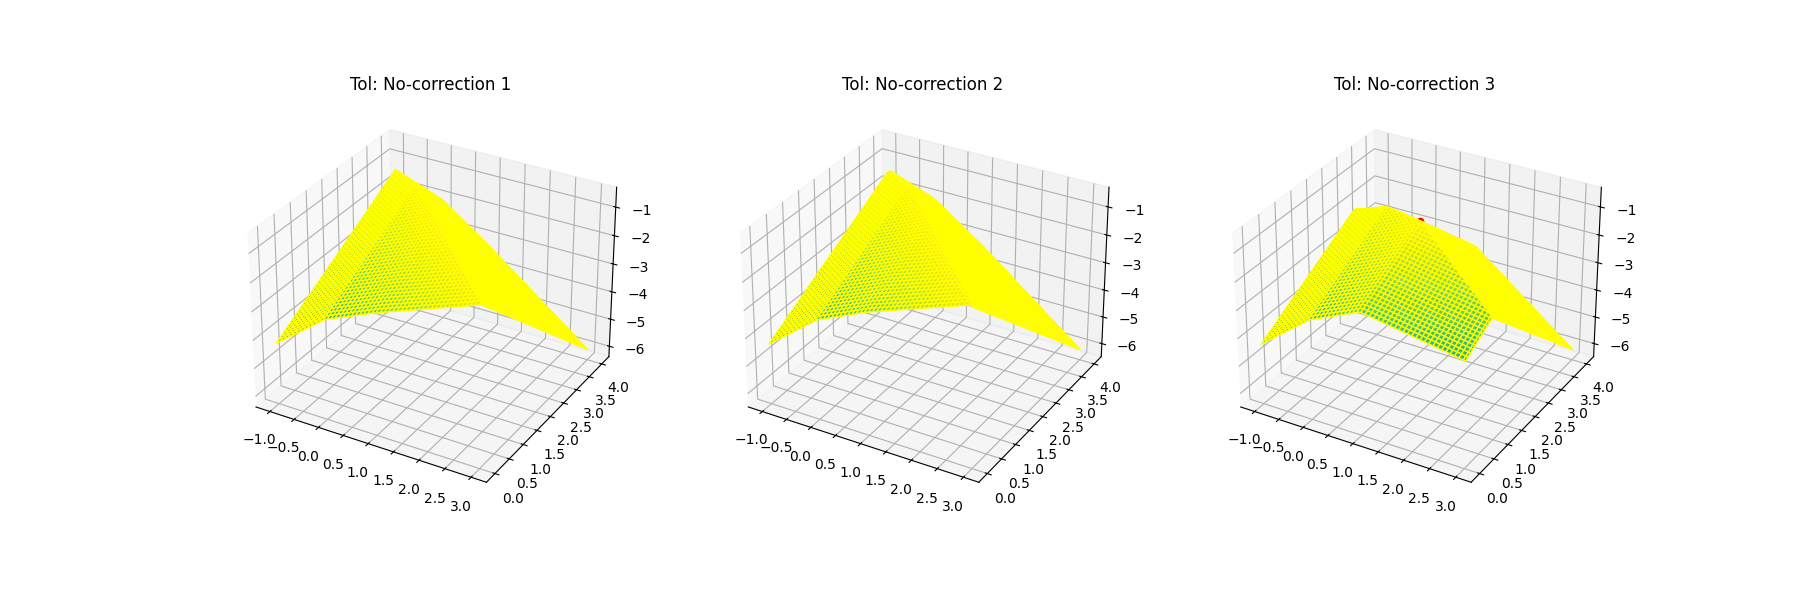
\includegraphics[scale=0.4]{No-corrections.png}
\caption{График $Tol(x, \mathbf{A}, \mathbf{b})$ без коррекции}
\end{figure}

\newpage
\subsection{b-коррекция}
Для $b$-коррекции для каждого случая выбрали константу $K=5$.\\

\begin{center}
\begin{tabular}{|c|c|c|c|c|}
\hline
$\mathbf{A}$&$\mathbf{b}$&$\mathbf{b}_{corr}$&$max{Tol(x, \mathbf{A}, \mathbf{b}_{corr})}$& $argmax{Tol}$\\
\hline
$\begin{pmatrix}
    [0.65, 1.25] & [0.70, 1.3] \\
    [0.75, 1.35] & [0.70, 1.3]
\end{pmatrix}$&$\begin{pmatrix}
    [2.75, 3.15] \\
    [2.85, 3.25]
\end{pmatrix}$&
$\begin{pmatrix}
    [-2.25, 8.15]\\
    [-2.15, 8.25]
\end{pmatrix}$
&4.3&[1,2]\\
\hline
$\begin{pmatrix}
    [0.65, 1.25] & [0.70, 1.3] \\
    [0.75, 1.35] & [0.70, 1.3] \\
    [0.8, 1.4] & [0.70, 1.3]
\end{pmatrix}$
&$\begin{pmatrix}
    [2.75, 3.15] \\
    [2.85, 3.25]\\
    [2.90, 3.3]
\end{pmatrix}$&
$\begin{pmatrix}
    [-2.25, 8.15]\\
    [-2.15, 8.25]\\
    [-2.1, 8.3]
\end{pmatrix}$
&4.3&[1,2]\\
\hline
$\begin{pmatrix}
    [0.65, 1.25] & [0.70, 1.3] \\
    [0.75, 1.35] & [0.70, 1.3] \\
    [0.8, 1.4] & [0.70, 1.3] \\
    [-0.3, 0.3] & [0.70, 1.3]
\end{pmatrix}$&$\begin{pmatrix}
    [2.75, 3.15] \\
    [2.85, 3.25]\\
    [2.90, 3.3] \\
    [1.8,2.2]
\end{pmatrix}$&
$\begin{pmatrix}
    [-2.25, 8.15]\\
    [-2.15, 8.25]\\
    [-2.1, 8.3]\\
    [-3.2, 7.2]
\end{pmatrix}$
&4.3&[1,2]\\
\hline
\end{tabular}
\end{center}

\begin{figure}[!htb]
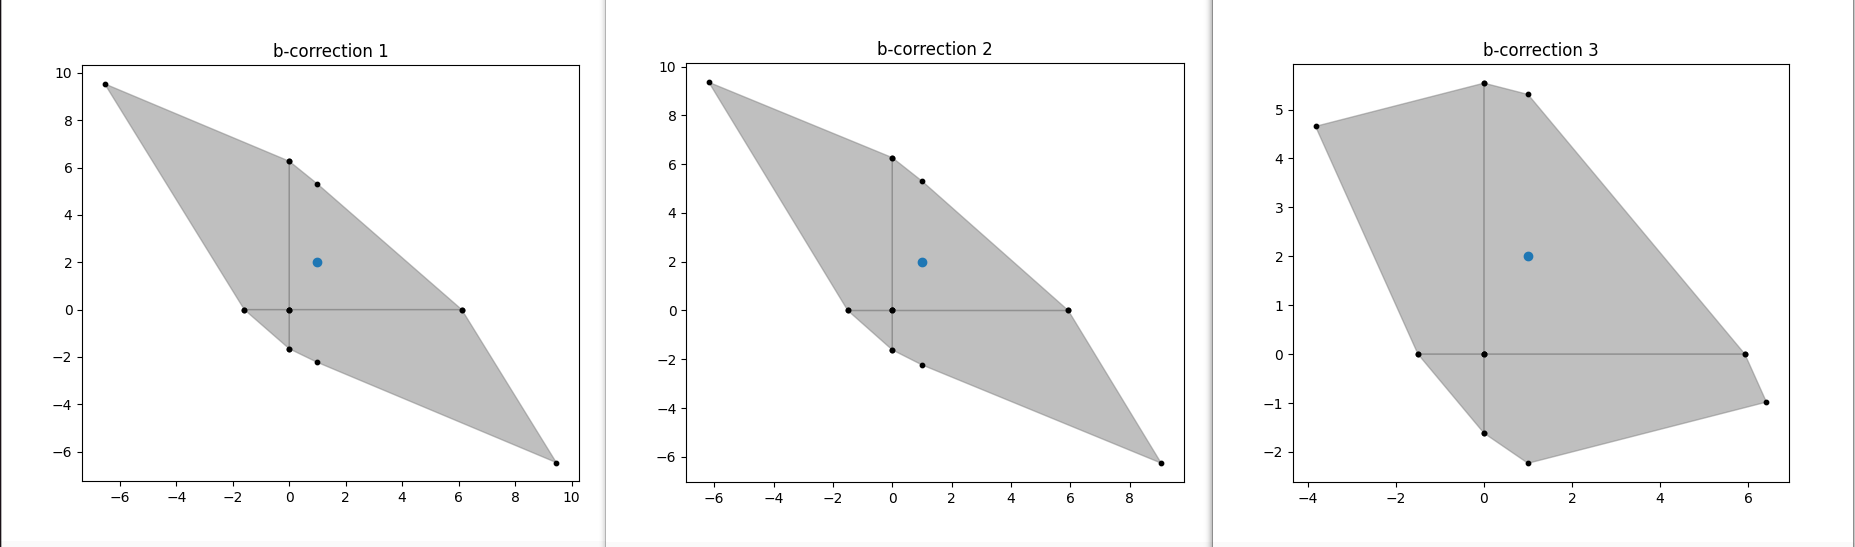
\includegraphics[scale=0.3]{Corr-b-correction.png}
\caption{Допусковое множество после $b$-коррекции}
\end{figure}

\begin{figure}[!htb]
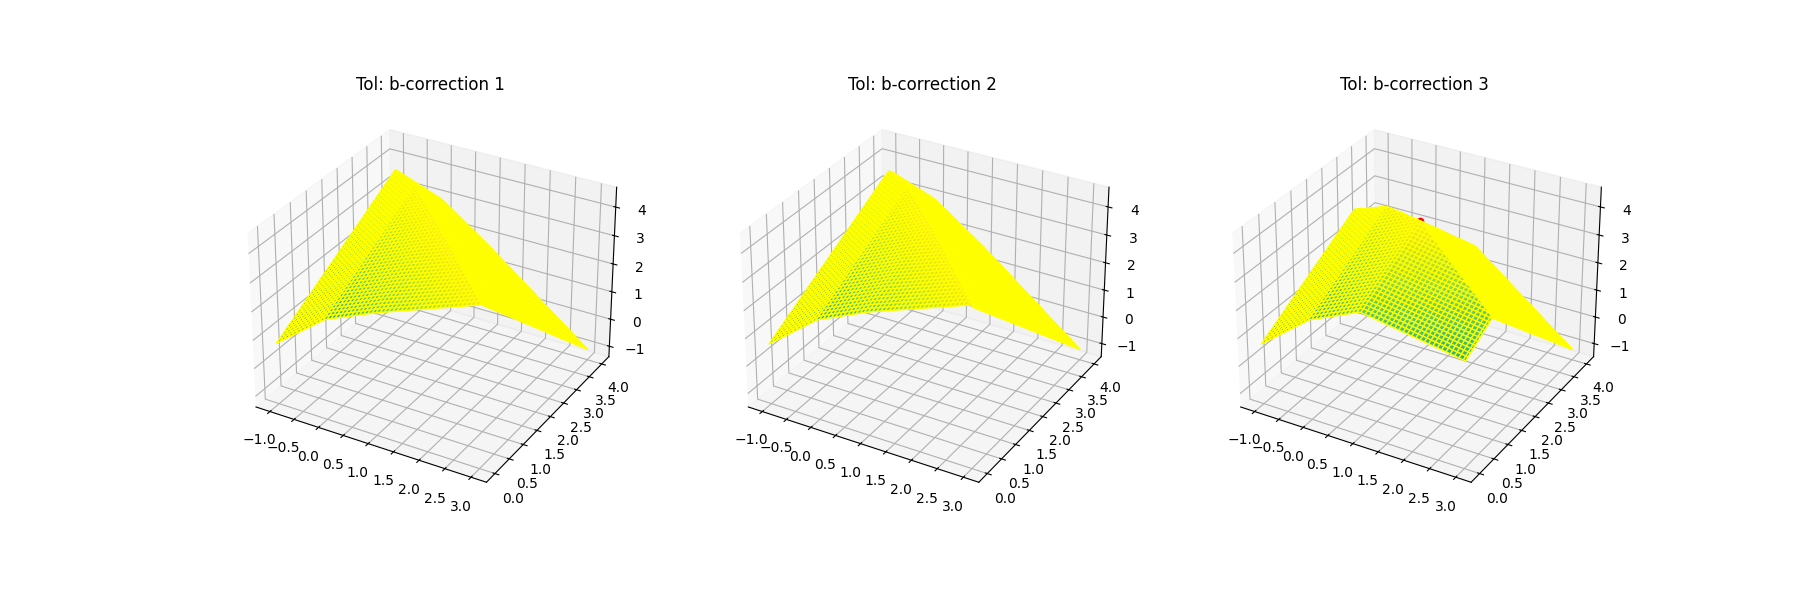
\includegraphics[scale=0.4]{b-corrections.png}
\caption{График $Tol(x, \mathbf{A}, \mathbf{b})$ после $b$-коррекции}
\end{figure}


\newpage
\subsection{A-коррекция}
  В случае \( A \)-коррекции для нахождения интервала допустимых значений \( e \) необходимо выполнить следующие действия для всех матриц:

  \begin{equation*}
    T = \text{Tol}(\tau, \mathbf{A}, \mathbf{b}) = -0.7 \Rightarrow |T| = 0.7,
  \end{equation*}
  \begin{equation*}
    \tau = \text{Arg} \max_{x \in \mathbb{R}^n}
    \text{Tol}(x, \mathbf{A}, \mathbf{b}) = (1, 2)^T \Rightarrow
    |\tau_1| = 1, \ |\tau_2| = 2.
  \end{equation*}

  где можно найти точную матрицу

  \begin{equation*}
    \text{rad} A = \begin{pmatrix}
      0.3 & 0.3 \\
      0.3 & 0.3 \\
      0.3 & 0.3 \\
      0.3 & 0.3
    \end{pmatrix}.
  \end{equation*}

  Далее решаем систему:

  \begin{equation*}
    \begin{cases}
      0 \leqslant e \leqslant 0.3, \\
      e + 2e = K \geqslant |T| = 0.7
    \end{cases} \Rightarrow 0.23 \leqslant e \leqslant 0.3.
  \end{equation*}

  Выберем \( e_{\text{mid}} = \frac{0.23 + 0.3}{2} = 0.255 \). 

  Максимум со значением \( T = 0.1 \) расположен в точке
  \( \tau = (1, 2)^T \).
\begin{center}
\begin{tabular}{|c|c|c|c|c|}
\hline
$\mathbf{A}$&$\mathbf{b}$&$\mathbf{A}_{corr}$&$max{Tol}$& $argmax{Tol}$\\
\hline
$\begin{pmatrix}
    [0.65, 1.25] & [0.70, 1.3] \\
    [0.75, 1.35] & [0.70, 1.3]
\end{pmatrix}$&$\begin{pmatrix}
    [2.75, 3.15] \\
    [2.85, 3.25]
\end{pmatrix}$&
$\begin{pmatrix}
    [0.92, 0.98] & [0.97, 1.03]\\
    [1.02, 1.08] & [0.97, 1.03]\\
\end{pmatrix}$
&0.099&[1,2]\\
\hline
$\begin{pmatrix}
    [0.65, 1.25] & [0.70, 1.3] \\
    [0.75, 1.35] & [0.70, 1.3] \\
    [0.8, 1.4] & [0.70, 1.3]
\end{pmatrix}$
&$\begin{pmatrix}
    [2.75, 3.15] \\
    [2.85, 3.25]\\
    [2.90, 3.3]
\end{pmatrix}$&
$\begin{pmatrix}
    [0.92, 0.98]&[0.97, 1.03] \\
    [1.02, 1.08]&[0.97, 1.03] \\
    [1.07, 1.13]&[0.97, 1.03]
\end{pmatrix}$
&0.099&[1,2]\\
\hline
$\begin{pmatrix}
    [0.65, 1.25] & [0.70, 1.3] \\
    [0.75, 1.35] & [0.70, 1.3] \\
    [0.8, 1.4] & [0.70, 1.3] \\
    [-0.3, 0.3] & [0.70, 1.3]
\end{pmatrix}$&$\begin{pmatrix}
    [2.75, 3.15] \\
    [2.85, 3.25]\\
    [2.90, 3.3] \\
    [1.8,2.2]
\end{pmatrix}$&
$\begin{pmatrix}
    [0.92, 0.98]&[0.97, 1.03]\\
    [1.02, 1.08]&[0.97, 1.03]\\
    [1.07, 1.13]&[0.97, 1.03]\\
    [-0.03, 0.03]&[0.97, 1.03]
\end{pmatrix}$
&0.099&[1,2]\\
\hline
\end{tabular}
\end{center}

\newpage
\begin{figure}[!htb]
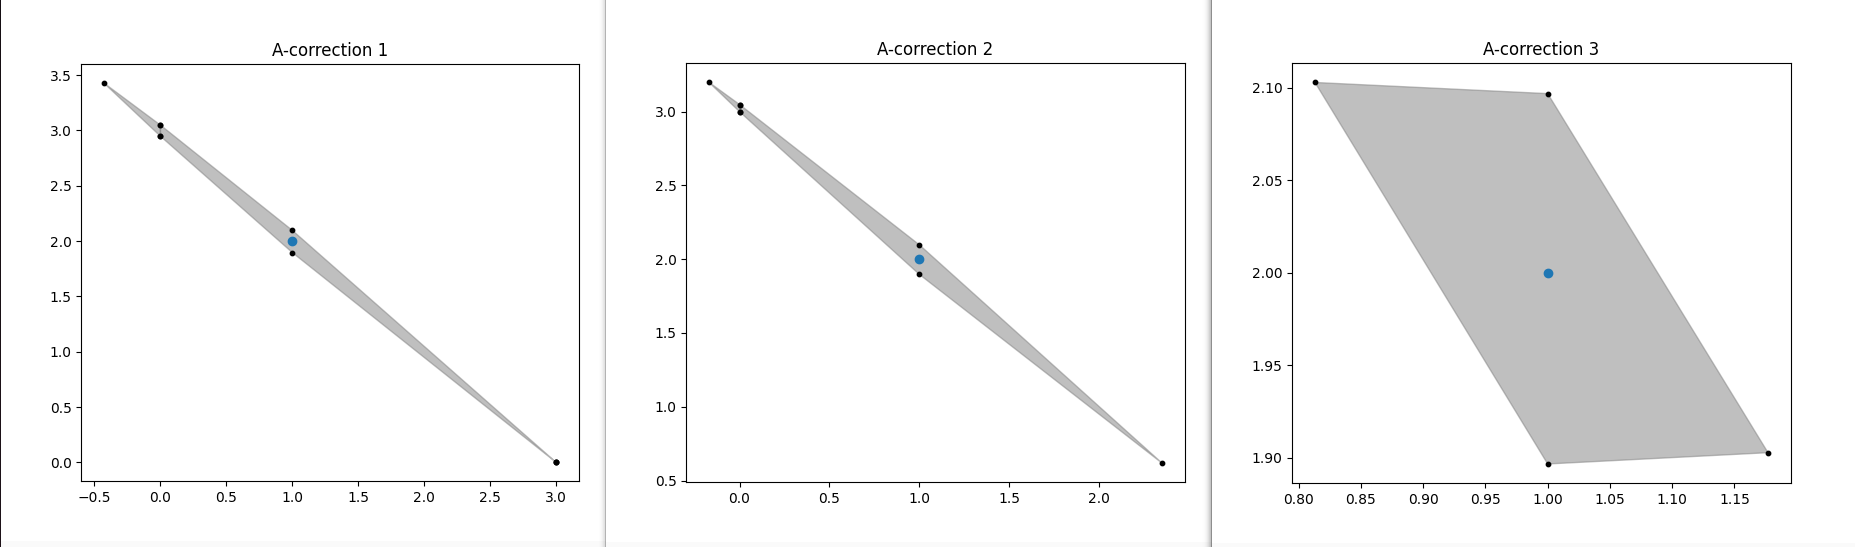
\includegraphics[scale=0.3]{Corr-A-correction.png}
\caption{Допусковое множество после $A$-коррекции}
\end{figure}


\begin{figure}[!htb]
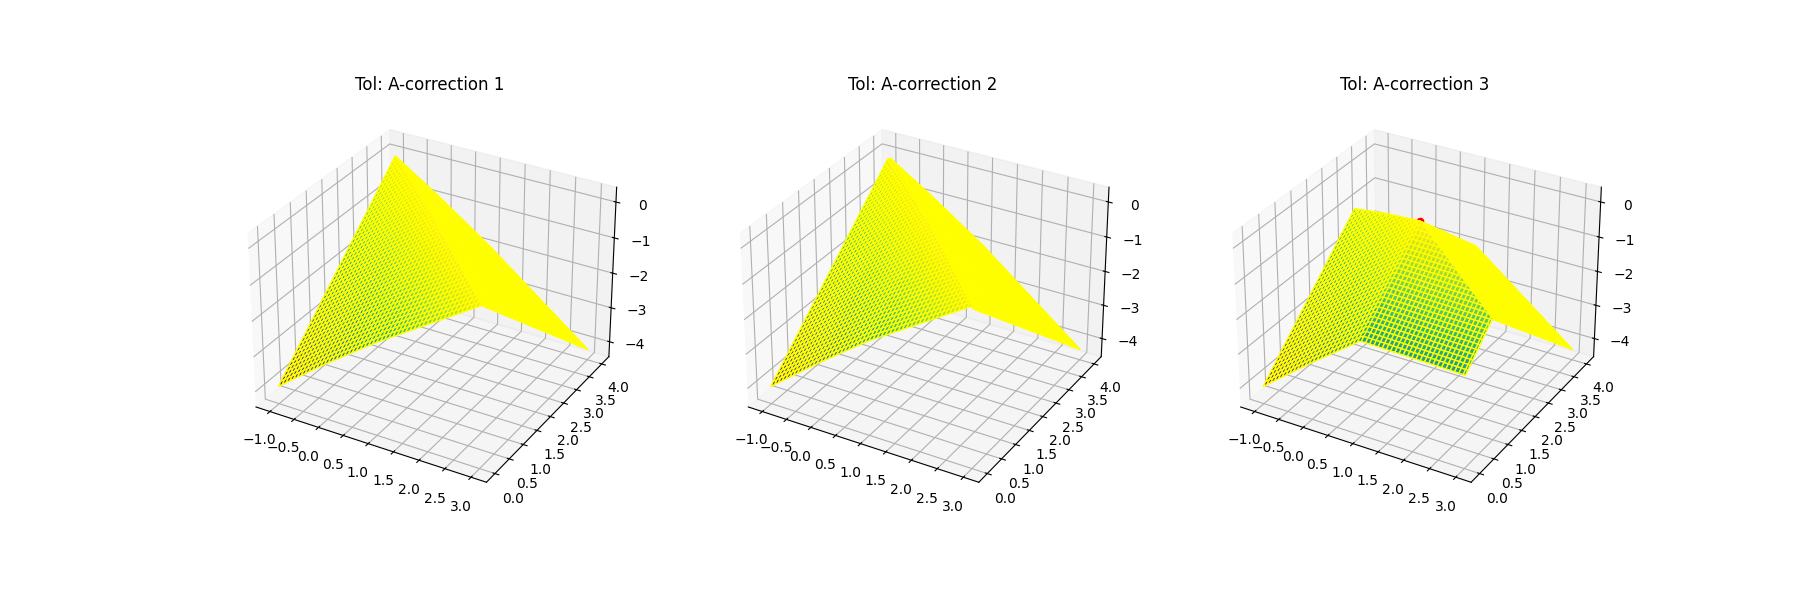
\includegraphics[scale=0.4]{A-corrections.png}
\caption{График $Tol(x, \mathbf{A}, \mathbf{b})$ после $A$-коррекции}
\end{figure}

\newpage
\subsection{Ab-коррекция}
Сначала производилась коррекция матрица $\mathbf{A}$, после коррекция вектора правой части $\mathbf{b}$ c K=5.

\begin{center}
\centering\small
\begin{tabular}{|c|c|c|c|c|c|}
\hline
$\mathbf{A}$&$\mathbf{b}$&$\mathbf{A}_{corr}$&$\mathbf{b}_{corr}$&$max{Tol}$& $argmax{Tol}$\\
\hline
$\begin{pmatrix}
    [0.65, 1.25] & [0.70, 1.3] \\
    [0.75, 1.35] & [0.70, 1.3]
\end{pmatrix}$&$\begin{pmatrix}
    [2.75, 3.15] \\
    [2.85, 3.25]
\end{pmatrix}$&
$\begin{pmatrix}
    [0.92, 0.98] & [0.97, 1.03]\\
    [1.02, 1.08] & [0.97, 1.03]\\
\end{pmatrix}$
&
$\begin{pmatrix}
    [2.75, 3.15] \\
    [2.85, 3.25]
\end{pmatrix}$
&0.099&[1,2]\\
\hline
$\begin{pmatrix}
    [0.65, 1.25] & [0.70, 1.3] \\
    [0.75, 1.35] & [0.70, 1.3] \\
    [0.8, 1.4] & [0.70, 1.3]
\end{pmatrix}$
&$\begin{pmatrix}
    [2.75, 3.15] \\
    [2.85, 3.25]\\
    [2.90, 3.3]
\end{pmatrix}$&
$\begin{pmatrix}
    [0.92, 0.98]&[0.97, 1.03] \\
    [1.02, 1.08]&[0.97, 1.03] \\
    [1.07, 1.13]&[0.97, 1.03]
\end{pmatrix}$&$\begin{pmatrix}
    [2.75, 3.15] \\
    [2.85, 3.25]\\
    [2.90, 3.3]
\end{pmatrix}$
&0.099&[1,2]\\
\hline
$\begin{pmatrix}
    [0.65, 1.25] & [0.70, 1.3] \\
    [0.75, 1.35] & [0.70, 1.3] \\
    [0.8, 1.4] & [0.70, 1.3] \\
    [-0.3, 0.3] & [0.70, 1.3]
\end{pmatrix}$&$\begin{pmatrix}
    [2.75, 3.15] \\
    [2.85, 3.25]\\
    [2.90, 3.3] \\
    [1.8,2.2]
\end{pmatrix}$&
$\begin{pmatrix}
    [0.92, 0.98]&[0.97, 1.03]\\
    [1.02, 1.08]&[0.97, 1.03]\\
    [1.07, 1.13]&[0.97, 1.03]\\
    [-0.03, 0.03]&[0.97, 1.03]
\end{pmatrix}$&$\begin{pmatrix}
    [2.75, 3.15] \\
    [2.85, 3.25]\\
    [2.90, 3.3] \\
    [1.8,2.2]
\end{pmatrix}$&0.099&[1,2]\\
\hline
\end{tabular}
\end{center}

\begin{figure}[!htb]
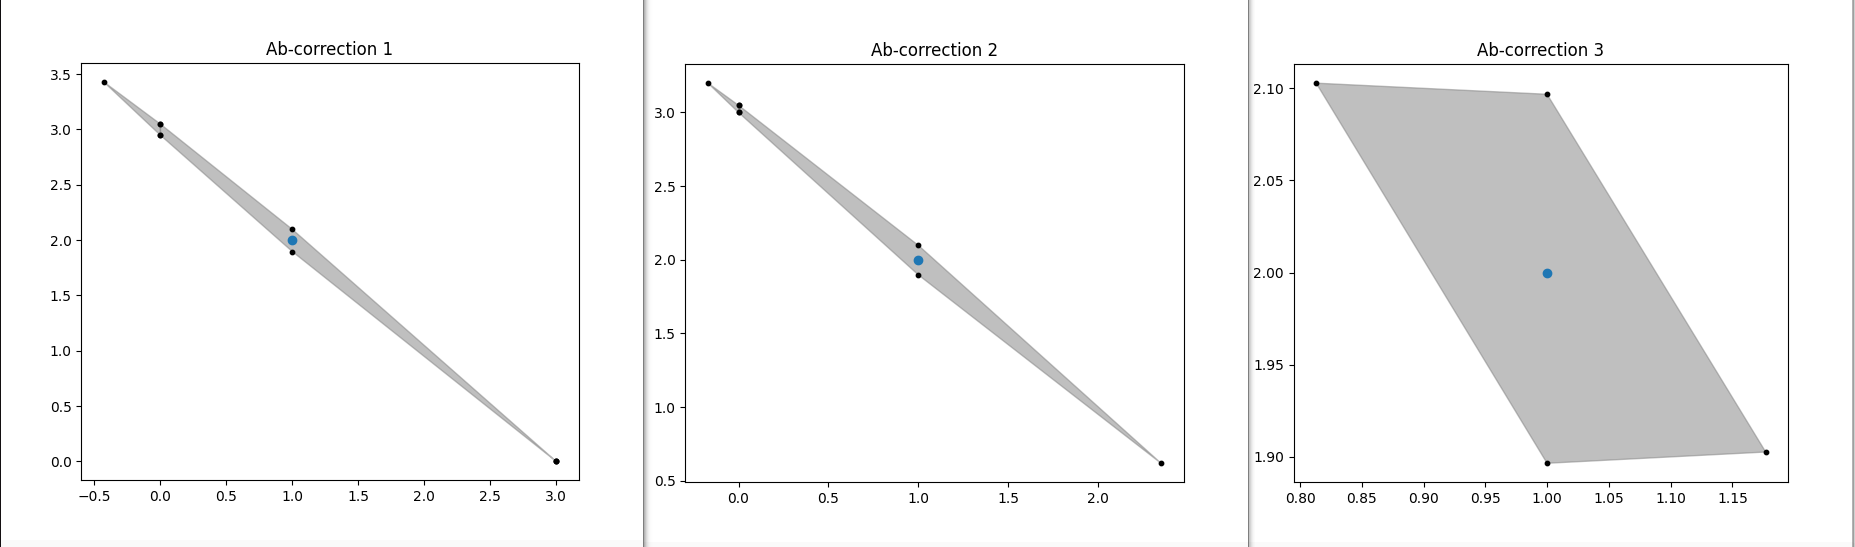
\includegraphics[scale=0.3]{Corr-Ab-correction.png}
\caption{Допусковое множество после $Ab$-коррекции}
\end{figure}

\begin{figure}[!htb]
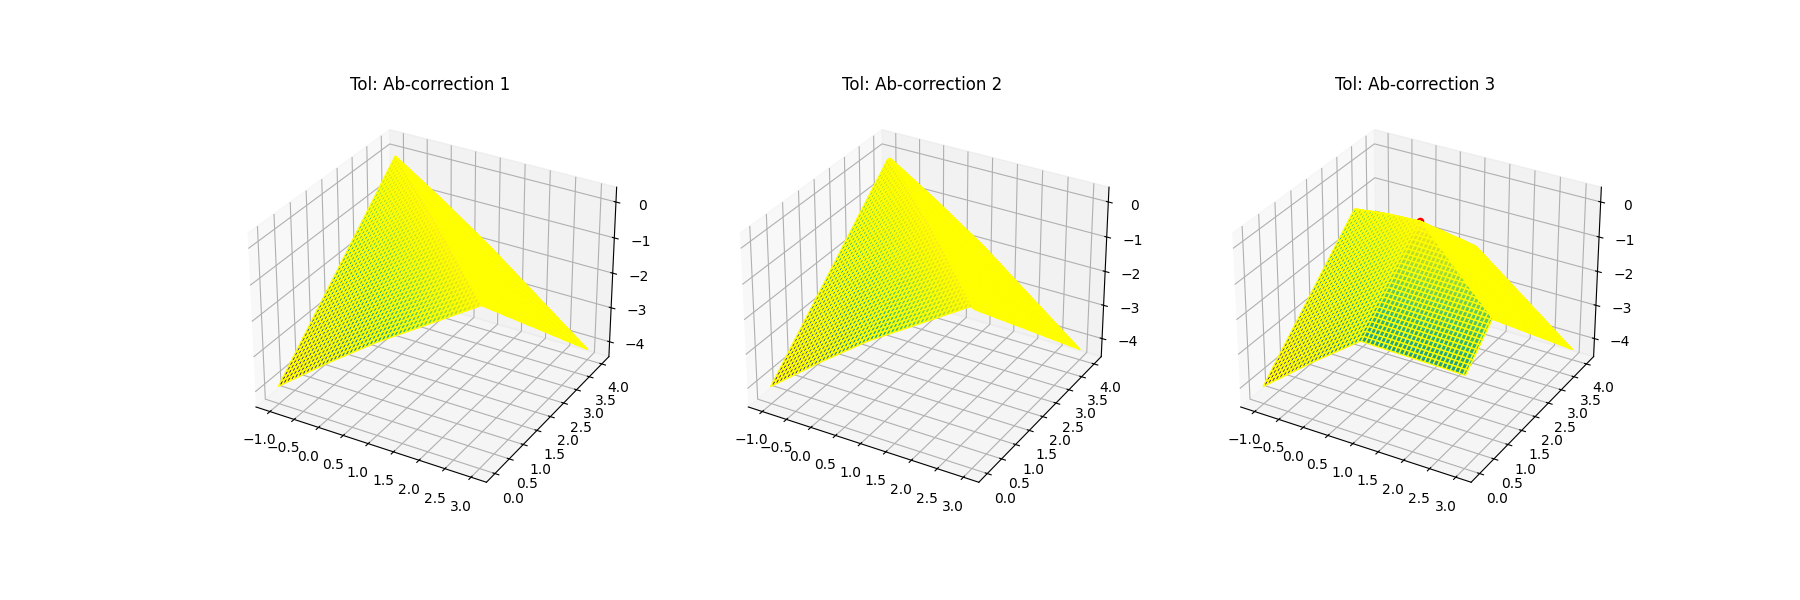
\includegraphics[scale=0.4]{Ab-corrections.png}
\caption{График $Tol(x, \mathbf{A}, \mathbf{b})$ после $Ab$-коррекции}
\end{figure}


\newpage
\section{Выводы}
\begin{itemize}
    \item В ходе лабораторной работы было установлено, что для исходных ИСЛАУ допусковое множество решений является пустым: максимум распознающего функционала $max Tol = $ и сообщающее максимум значение $argmax = $. Из отрицательности значения $max Tol$ следует несовместность исходной системы.
    \item Для достижения совместности систем были применены методы коррекции правой части (b-коррекция), левой части (A-коррекция) и коррекция обеих частей (Ab-коррекция).\\ 
    В результате всех видов коррекции исходных матриц были получены положительные максимумы распознающего функционала. Заметим, что в ходе Ab-коррекции совместность системы была достигнута засчёт коррекции левой части, что можно проследить по результатам, вынесенным в таблицах. 
    \item Из графиков допусковых множеств и графиков распознающего функционала видно, как в результате разных видов коррекции меняется форма допусковых множеств и форма поверхности Tol(x). Кроме того, факт смещения максимума распознающего функционала подтверждает улучшение систем.
\end{itemize}

\section{GitHub}
Ссылка на репозиторий с кодом: \url{https://github.com/11AgReS1SoR11/Interval.git} \\

\section{Литература}
\begin{itemize}
    \item A.Н.Баженов. Интервальный анализ. Основы теории и учебные примеры. СПБПУ. 2020
    \item A.Н.Баженов., Н.В.Ермаков. Малоракурсная томография. Спб.: Политех-Пресс. 2023.  
\end{itemize}

\end{document}
